

\documentclass{beamer}
\usepackage[utf8]{inputenc}
\usepackage[T1]{fontenc}

\usepackage{amsmath}
\usepackage{mathtools}
\usepackage{amsthm}
\usepackage{amssymb}
\usepackage{tcolorbox}
\tcbuselibrary{theorems}
\usepackage{tikz-cd}
\usepackage{xparse}
\usepackage{adjustbox}
\usepackage{braket}



\usepackage{tabularx}

%\newcommand{\cat}[1]{\mathcal{#1}}



\title{The Wightman Axioms for Hopf-Frobenius Modules}

\author{Matt Alexander}
\usetheme{queer}


%\newcommand{\newthought}[1]{\medskip\noindent\fbox{{#1}}}




%=================================
% Colourblind-friendly colours
%=================================


% 6 Colour Attempt Feb 27, 2024


\definecolor{lemmacolour}{RGB}{0, 0, 153} 


\definecolor{propcolour}{RGB}{138, 10,0}

\definecolor{definitioncolour}{RGB}{100, 100, 100}

\definecolor{examplecolour}{RGB}{62,217,141}

\definecolor{conjecturecolour}{RGB}{235, 160, 215}

\definecolor{theoremcolour}{RGB}{255, 240, 0}



%============================
% 5 Colour Attempt
%============================



%\definecolor{corolcolour}{RGB}{0, 114, 178}


%Compare this one and examplecolor on tritanopia
%\definecolor{lemmacolour}{RGB}{0, 114, 178} 
%
%
%\definecolor{propcolour}{rgb}{0.6, 0.0,0.0}
%
%
%\definecolor{theoremcolour}{rgb}{1.0, 0.84, 0.0}
%
%
%
%
%\definecolor{examplecolour}{RGB}{59,191,143}
%
%\definecolor{definitioncolour}{rgb}{0.75, 0.75, 0.75}



%============================
% Theorem Environments
%============================


\usepackage{}



\newenvironment{proof-lemma}
    {\begin{mdframed}[linewidth=3, linecolor=lemmacolour,topline=false,rightline=false,bottomline=false]
\begin{proof}
}{
\end{proof}
\end{mdframed}}


\newenvironment{proof-prop}
    {\begin{mdframed}[linewidth=3, linecolor=propcolour,topline=false,rightline=false,bottomline=false]
\begin{proof}
}{
\end{proof}
\end{mdframed}}


\newenvironment{proof-theorem}
    {\begin{mdframed}[linewidth=3, linecolor=theoremcolour,topline=false,rightline=false,bottomline=false]
\begin{proof}
}{
\end{proof}
\end{mdframed}}

\newenvironment{proof-corol}
    {\begin{mdframed}[linewidth=3, linecolor=lemmacolour,topline=false,rightline=false,bottomline=false]
\begin{proof}
}{
\end{proof}
\end{mdframed}}

\newenvironment{defframe}
    {\begin{mdframed}[linewidth=3, linecolor=definitioncolour,topline=false,rightline=false,bottomline=false]
}{
\end{mdframed}}

\newenvironment{exampleframe}
    {\begin{mdframed}[linewidth=3, linecolor=examplecolour,topline=false,rightline=false,bottomline=false]
}{
\end{mdframed}}

\newenvironment{conjecframe}
    {\begin{mdframed}[linewidth=3, linecolor=conjecturecolour,topline=false,rightline=false,bottomline=false]
}{
\end{mdframed}}



%============================

%\newtcbtheorem[number within=section]{theorem}{\color{black}Theorem}%
%{colback=theoremcolour!5,colframe=theoremcolour,fonttitle=\bfseries}{th}





%==========================================



%==============================================
% Theorems v.2
%==============================================


\newtcbtheorem[number within=section]{deff}{Definition}%
{colback=definitioncolour!5, colframe=definitioncolour,fonttitle=\bfseries}{th}


\newtcbtheorem[number within=section]{lemm}{Lemma}%
{colback=lemmacolour!5,colframe=lemmacolour!95!black,fonttitle=\bfseries}{th}



% Had to change this just for this presentation, so we didn't get prop 0.1, since there are no 'sections' in a beamer presentation.

\newtcbtheorem{prop}{Proposition}%
{colback=propcolour!5,colframe=propcolour,fonttitle=\bfseries}{th}



\newtcbtheorem[number within=section]{corol}{Corollary}%
{colback=corolcolour!5,colframe=corolcolour!95!black,fonttitle=\bfseries}{th}

\newtcbtheorem[number within=section]{exam}{Example}%
{colback=examplecolour!5,colframe=examplecolour,{fonttitle=\bfseries \color{black}}}{th}



\newtcbtheorem[number within=section]{conj}{Conjecture}%
{colback=conjecturecolour!5,colframe=conjecturecolour,{fonttitle=\bfseries \color{black}}}{th}


\newtcbtheorem[number within=section]{thm}{\color{black}Theorem}%
{colback=theoremcolour!5,colframe=theoremcolour,{fonttitle=\bfseries \color{black}},
label type=theorem}{thm}



%==============================================
% Theorems v.1
%==============================================


%\newtcbtheorem[number within=section]{definition}{Definition}%
%{colback=definitioncolour!5,colframe=definitioncolour!50!black,fonttitle=\bfseries}{th}
%
%
%\newtcbtheorem[number within=section]{lemma}{Lemma}%
%{colback=lemmacolour!5,colframe=lemmacolour!95!black,fonttitle=\bfseries}{th}
%
%
%\newtcbtheorem[number within=section]{prop}{Proposition}%
%{colback=propcolour!5,colframe=propcolour,fonttitle=\bfseries}{th}
%
%
%
%\newtcbtheorem[number within=section]{corollary}{Corollary}%
%{colback=corolcolour!5,colframe=corolcolour!95!black,fonttitle=\bfseries}{th}
%
%\newtcbtheorem[number within=section]{example}{Example}%
%{colback=examplecolour!5,colframe=examplecolour!90!black,fonttitle=\bfseries}{th}
%
%
%
%\newtcbtheorem[number within=section]{conjecture}{Conjecture}%
%{colback=conjecturecolour!5,colframe=conjecturecolour!90!black,fonttitle=\bfseries}{th}
%
%
%\newtcbtheorem[number within=section]{theorem}{\color{black}Theorem}%
%{colback=theoremcolour!5,colframe=theoremcolour,{fonttitle=\bfseries \color{black}},
%label type=theorem}{thm}








%\usepackage[demo]{graphicx}
\usepackage{wallpaper}
\usepackage{wrapfig,booktabs}

\usepackage{fancyhdr}
\usepackage{lettrine}

\usepackage{mdframed}

\usepackage{cancel}

%\usepackage{geometry}
%\geometry{
%tmargin=5cm, 
%bmargin=5cm, 
%lmargin=5cm, 
%rmargin=3cm,
%headheight=1.5cm,
%headsep=0.8cm,
%footskip=0.5cm}


\usepackage{tabularx}

\usepackage{braket}




%=====================
% MATH
%=====================

\usepackage{amsmath}
\usepackage{mathtools}
\usepackage{amsthm}
\usepackage{amssymb}
\usepackage{tcolorbox}
\tcbuselibrary{theorems}
\usepackage{tikz-cd}
\usepackage{xparse}

% To get a get a nice curvy arrow to talk about paths
\DeclareSymbolFont{lasy}{U}{lasy}{m}{n}
\SetSymbolFont{lasy}{bold}{U}{lasy}{b}{n}
\DeclareMathSymbol\leadsto{\mathrel}{lasy}{"3B}



% To have arrow heads in the middle
\usetikzlibrary{decorations.markings, arrows.meta}
\tikzset{
    marrow/.style={decoration={markings,mark=at position 0.5 with {\arrow{#1}}}, postaction=decorate}
}


%\usepackage[colorlinks=true]{hyperref}

\usepackage[nameinlink]{cleveref} % Better references to lemmas etc. The nameinlink makes all of 'Theorem 1' clickable


%\usepackage{titling} %Lets you have more than one title in a document
% But this won't work with ams articles, so I'll need to add it in separately for my own work and comment it out for research articles


\usepackage{adjustbox}



\usepackage[nointegrals]{wasysym}

\usepackage{fontawesome} % really cool fonts like morph and obj
\usepackage{tikz}



%========================
% COMMANDS
%========================


\newcommand{\Def}[1]{\textbf{\boldmath{#1}}}



%Field Theory
\newcommand{\exten}[2]{{#2}_{#1}}



\newcommand{\colim}{\operatorname{colim}}

\newcommand{\tabitem}{~~\llap{\textbullet}~~}

\newcommand{\newthought}[1]{\medskip\noindent\fbox{{#1}}}


\newcommand{\abs}[1]{| #1 |}

\newcommand{\cat}[1]{\mathcal{#1}}


\newcommand{\coker}{\operatorname{coker}}

\newcommand{\im}{\operatorname{Im}}

\newcommand{\const}{\text{\faAsterisk}}


\newcommand{\obj}{\text{\faCube}}

\newcommand{\morph}{\text{\faLocationArrow}}

\newcommand{\mor}[2]{\text{Mor}(#1, #2)}

\newcommand{\nbh}[1]{\mathcal{N}_{#1}} % The set of neighbourhoods around $x$.


\newcommand{\twist}{\text{\faRefresh}}


%================================
% HOMOTOPY / MODEL CATEGORIES
%=================================

\newcommand{\cyl}{\text{\faDatabase}}

\newcommand{\paths}{\text{\faPencilSquareO }}


%
%\newcommand{\bnbh}[1]{\mathcal{B}_{#1}}
%
%\newcommand{\base}[1]{\langle \cdot #1 \cdot \rangle}

\newcommand{\norm}[1]{\left\lVert #1 \right\rVert}

\newcommand{\gen}[1]{\left\langle #1 \right\rangle}

\newcommand{\triforce}{\resizebox{1em}{!}{
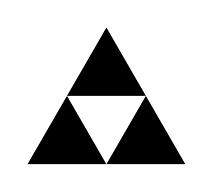
\begin{tikzpicture}
\fill[black] (0,0)  -- +(2,0) -- +(60:2) -- cycle;
\fill[white]  (60:1) -- +(1,0)  -- (1,0) -- cycle;
\end{tikzpicture}
}}





\begin{document}


\begin{frame}
\titlepage
\end{frame}



%===================
% SLIDE 1
%===================







%===================
% SLIDE 2
%===================



\begin{frame}

\frametitle{Definition of Frobenius Algebras}

%\framesubtitle{Part 3 --- Equivalences}

A Frobenius algebras is a unital associative $k$-algebra with a pairing $\gen{\cdot, \cdot}: F \otimes F \to k$, such that

\begin{itemize}
\item \newthought{Non-degenerate: } If $\gen{x,y} = 0$ for all $y$, then $x = 0$. Similarly, $\gen{x,y} = 0$ for all $x$ implies $y=0$.

\item \fbox{Associativity: } $\gen{xy,z} = \gen{x,yz}$, or in the complex case, $\gen{xy,z} = \gen{x, y^* z}$.
\end{itemize}


\newthought{Equivalently: } A linear functional $\varepsilon: F \to k$, that satisfies the non-degeneracy condition
\begin{equation*}
\gen{x,y} = \varepsilon(xy) \quad \gen{x,y} = \varepsilon(x^* y)
\end{equation*}


\end{frame}


%===================
% SLIDE 1
%===================



%===================
% SLIDE 2
%===================



\begin{frame}
\frametitle{Frobenius Algebras}

\framesubtitle{Examples}



\begin{tabularx}{\textwidth}{lll>{\raggedright\arraybackslash}X}
\toprule
Space & $\mu$ & $\gen{\cdot, \cdot}$ 
\\
\midrule
\\
$C_c^{\infty}(X)$ & Pointwise & $\gen{f,g} = \int f^* g$ \\
Schwartz functions $\cat{S}$ & Pointwise & $\gen{f,g} = \int f^* g$
\\
\\
$\mathbb{R}^n$ w/ basis $\{ e_i \}$ & $e_i e_j = \delta_{ij} e_i$ & $\gen{e_i,e_j} = \delta_{ij}$ \\
Hilbert space w/ basis $\{ e_i \}$ & $e_i e_j = \delta_{ij} e_i$ & $\gen{e_i,e_j} = \gen{e_i, e_j}_H$  \\
\\
$kG$ (finite group) & Group mult. & $\gen{g,h} = \delta_{gh, 1}$ 
\\
\bottomrule
\end{tabularx}

\medskip


\begin{equation*}
\cat{S} = \{ f \in C^{\infty}(\mathbb{R}^n, \mathbb{C}) \mid \sup_{x} \abs{x^\alpha D^\beta f(x)} < \infty, \forall \alpha, \beta \}
\end{equation*}



\end{frame}

%===================
% SLIDE 3
%===================



\begin{frame}
\frametitle{Hopf Algebras}

\framesubtitle{Definition}

A Hopf algebra is a unital associative $k$-algebra, $H$, with maps 

\medskip

\begin{itemize}
\item \fbox{Comultiplication: } $\Delta: H \to H \otimes H$

\item \fbox{Counit: } $\varepsilon: H \to k$

\item \fbox{Antipode: } An involution $S: H \to H$
\end{itemize}
which satisfy appropriate compatibility conditions.

\medskip

\adjustbox{center}{
\begin{tikzpicture}
  \node {$H$}
    child {node {$\mu$}
    		child {node {$H$}}
    		child {node {$H$}}
    	};
\end{tikzpicture}
\quad
\raisebox{6pt}{
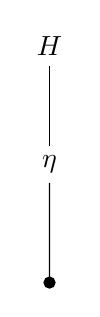
\begin{tikzpicture}
  \node {$H$}
    child {node {$\eta$}
    		child {[fill] circle (2pt)}
    	};
\end{tikzpicture}}
\quad
\begin{tikzpicture}
  \node {$H$} [grow'=up]
    child {node {$\Delta$}
    		child {node {$H$}}
    		child {node {$H$}}
    	};
\end{tikzpicture}
\quad
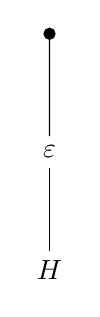
\begin{tikzpicture}[grow'=up]
  \node {$H$}
    child {node {$\varepsilon$}
    		child {[fill] circle (2pt)}
    	};
\end{tikzpicture}
\quad
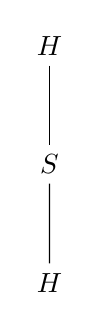
\begin{tikzpicture}
  \node {$H$}
    child {node {$S$}
    		child {node {$H$}}
    	};
\end{tikzpicture}
}

%
%\begin{tikzpicture}
%  \node[fill, circle] {}
%    child {[fill] circle (2pt)}
%    child {[fill] circle (2pt)} {child {[fill] circle (2pt)}}
%    child {[fill] circle (2pt)};
%\end{tikzpicture}

\end{frame}










\begin{frame}


\frametitle{Hopf Algebras}
%

\framesubtitle{Examples}

\begin{tabularx}{\textwidth}{lll>{\raggedright\arraybackslash}X}
\toprule
Space & $\Delta$ & $\varepsilon$
\\
\midrule
\\
$kG$  & $\Delta g = g \otimes g$ & $\varepsilon(g) = 1$ \\
\\
Tensor alg. $T(X)$ & $\Delta x = x \otimes 1 + 1 \otimes x$ & $\varepsilon(x) = 0$ \\
Symmetric alg. $S(X)$ & $\Delta x = x \otimes 1 + 1 \otimes x$ & $\varepsilon(x) = 0$ \\
Univ. Env. Alg. $U(\mathfrak{g})$ & $\Delta x = x \otimes 1 + 1 \otimes x$ & $\varepsilon(x) = 0$
\\
\\
$\Lambda(X)$ & $\Delta x = x \otimes 1 - 1 \otimes x$ & $\varepsilon(x) = 0$
\\
\bottomrule
\end{tabularx}

\medskip 

\newthought{Sweedler Notation: } Denote the comultiplication by
\begin{equation*}
\Delta x = \sum x_{(1)} \otimes x_{(2)}.
\end{equation*}

\end{frame}

%===================
% SLIDE 4
%===================


\begin{frame}

\frametitle{Hopf-Frobenius Modules}
\framesubtitle{Definition}

A left Hopf-Frobenius module is a pair $(H,F)$ where $H$ is a Hopf algebra, $F$ is a Frobenius algebra, such that the following conditions are satisfied:

\bigskip

\begin{itemize}

\item \fbox{Module: } $F$ is a left $H$-module.

\medskip

\item \fbox{Weak Cartan: }  $\sum \gen{g_{(1)} \cdot x, g_{(2)} \cdot y} = \varepsilon(g) \gen{x,y}$.

\medskip

\item \fbox{Antipode Condition: }  $\gen{S(g) \cdot x, y} = \gen{x, g \cdot y}$.

\end{itemize}





\end{frame}


\begin{frame}

\frametitle{Hopf-Frobenius Modules}
\framesubtitle{Example 1 --- Derivatives of Functions}


Take our Hopf algebra to be $k[\partial]$ and the Frobenius algebra to be $\cat{S}$, the space of Schwartz functions. This is an HF-module with

\bigskip

\begin{itemize}

\item \fbox{Action: } $\partial \cdot f = f'$, the derivative of $f$


\medskip

\item \fbox{Weak Cartan / Antipode: } Both of these conditions reduce to

\begin{equation*}
\int (\partial \cdot f) g  = - \int f (\partial \cdot g)
\end{equation*}
The \textbf{weak derivative} condition.
% $\gen{\partial f, g} + \gen{f, \partial g} = \varepsilon(\partial) \gen{f,g} = 0$. So
%\begin{equation}
%\int (\partial f) g + \int f (\partial g) = 0
%\end{equation}
%
%\item \fbox{Antipode: } $S(\partial) = - \partial$
\end{itemize}


\end{frame}



\begin{frame}

\frametitle{Hopf-Frobenius Modules}
\framesubtitle{Example 2 --- Operators on a Hilbert Space}

Let $F$ be a separable Hilbert space, and let $\{ A_i \}$ be a family of compact mutually-commuting \textit{skew-Hermitian} operators on $F$. Then we can find an orthonormal basis of simultaneous eigenvectors, $\{ e_k \}$. 

Take $(F, \{ e_k \})$ as our Frobenius algebra, and let $H = U(\{ A_i \} )$ be the universal enveloping algebra of the abelian Lie algebra generated by the $\{ A_i \}$. This is a HF-module where


\begin{itemize}

\item \fbox{Action: } $A_i \cdot e_k = A_i e_k = \alpha_{i}^k e_k$, the natural action of the Hermitian operators on the eigenvector basis.


\medskip

\item \fbox{Weak Cartan / Antipode: } Both of these conditions reduce to

\begin{equation*}
\gen{H x, y} = - \gen{x, Hy}
\end{equation*}
The \textbf{skew-Hermitian} condition.
\end{itemize}



\end{frame}





\begin{frame}

\frametitle{Hopf-Frobenius Modules}
\framesubtitle{Example 3 --- Lie Groups}


Consider the Lie group $U(n)$, and let $H$ be its group algebra over $\mathbb{C}$. Take $\mathbb{C}^n$ with basis $\{ e_i \}$ as our Frobenius algebra.

\bigskip

\begin{itemize}

\item \fbox{Action: } Left multiplication.


\medskip

\item \fbox{Weak Cartan / Antipode: } Both of these conditions reduce to

\begin{equation*}
\gen{g \cdot x, g \cdot y} = \gen{x,y}
\end{equation*}
The unitarity condition.

\end{itemize}




\end{frame}



%===================
% SLIDE 2
%===================



\begin{frame}


\frametitle{Hopf-Frobenius Modules}
%

\begin{tabularx}{\textwidth}{ll|ll>{\raggedright\arraybackslash}X}
\toprule
Frobenius & & Hopf
\\
\midrule
& & \\
States & \textbf{Hil} & Operators & $B(\textbf{Hil})$ \\
Functions & $\cat{S}$ & Derivatives & $\mathbb{C}[\partial_1, \ldots, \partial_n]$ \\
Space & $\mathbb{R}^{1,3}$ & Transformations & $\Lambda$
\\
&& \\
\bottomrule
\end{tabularx}



\end{frame}



%===================
% SLIDE 2
%===================




\begin{frame}
\frametitle{Wightman Axioms}
\framesubtitle{Relativistic Quantum Mechanics}


\begin{enumerate}
\item \fbox{Hilbert Space: } There is a separable Hilbert space of states $X$.

\item \fbox{Evolution: } There is a unitary representation of $SL(2, \mathbb{C})$ on $X$, which we denote $U(L,a)$

\item \fbox{Spectral Condition: } We can write $U(1,a) = \exp(i P^{\mu} a_\mu)$ and the eigenvalues of $P$ satisfy $p_0^2 - \sum_{i=1}^3 p_i^2 > 0$ and $p^0 > 0$.

\item \fbox{Vacuum: } There is a unique vector $\ket{0} \in X$ invariant under $U(L,a)$.
\end{enumerate}


\end{frame}





%===================
% SLIDE 2
%===================


\begin{frame}

\frametitle{Wightman Axioms}
\framesubtitle{Field Conditions}

\begin{enumerate}
\item \fbox{Dense Subset: } There is a dense subset $D \subseteq X$ which contains $\ket{0}$ and is mapped to itself by $U(L,a)$.

\item \fbox{Fields: } Quantum fields are operator-valued distributions on a Schwartz space, $\phi_i: \cat{S} \to B(D)$.

\item \fbox{Transformations: } There is an action of $SL(2)$ on the fields, $S(L)$ such that $U(L,a) \phi(x) U(L,a)^{-1} = S(L) \phi(L^{-1}(x - a))$

\item \fbox{Cyclic Vacuum: } The image of polynomials in $\phi_i(f)$ on $\ket{0}$ is dense in $X$.
\end{enumerate}


\end{frame}


%===================
% SLIDE 2
%===================


\begin{frame}

\frametitle{Wightman Axioms}
\framesubtitle{Microcausality Condition}

\begin{enumerate}

\item If $f,g \in \cat{S}$ have spacelike supports ($f(x) g(y) = 0$ for all $x,y$ with $d(x,y) \geq 0$) then $[\phi_i (f), \phi_j (g)]_{\pm}(v) = 0$ for all $v \in D$.

%[spacelike is negative distance]

\end{enumerate}

\end{frame}






%===================
% SLIDE 2
%===================




\begin{frame}
\frametitle{Hopf-Frobenius Wightman Axioms}
%\framesubtitle{Relativistic Quantum Mechanics}

A (weak) Hopf-Frobenius-Wightman QFT is a collection of Hopf algebras ($B(F_{\text{state}}), k SL(2)$)  and Frobenius algebras ($F_{\text{state}}, \cat{S}, \mathbb{R}^{1,3}$)  such that

\begin{enumerate}


\item \fbox{States and Evolution: } $(k SL(2),F_{\text{state}})$ forms a Hopf-Frobenius module.

\item \fbox{Vacuum: } There is a unit $1 \in F_{\text{state}}$, which is the unique element preserved by $k SL(2)$.

\item \fbox{Fields: } Quantum fields are linear maps $\cat{S} \to B(F_{\text{state}})$ and form a Frobenius algebra $F_{\text{field}}$.

\item \fbox{Field Transformations: } $(k SL(2),F_{\text{field}})$ forms a Hopf-Frobenius module.





\end{enumerate}


\end{frame}




\begin{frame}
\frametitle{Hopf-Frobenius Wightman Axioms}
\framesubtitle{Other Conditions}

\begin{enumerate}

\item \fbox{Dense Subset: } We can view $F_{\text{state}}$ as all of $D$.


\item \fbox{Cyclic Vacuum: } The image of polynomials in $\phi_i(f)$ on $\ket{0}$ is dense in $X$.


\item \fbox{Spectral Condition: } We can write $U(1,a) = \exp(i P^{\mu} a_\mu)$ and the eigenvalues of $P$ satisfy $p_0^2 - \sum_{i=1}^3 p_i^2 > 0$ and $p^0 > 0$.


\item \fbox{Causality: }  If $f,g \in \cat{S}$ have spacelike supports ($f(x) g(y) = 0$ for all $x,y$ with $d(x,y) \geq 0$) then $[\phi_i (f), \phi_j (g)]_{\pm}(v) = 0$ for all $v \in D$.


\end{enumerate}
\end{frame}

































\end{document}
%
%
%
%
%
%
